\chapter{The Father of Crypto Is Investing In This}

This chapter follows a School of Hard Knocks entrepreneurship segment curated by LazyingArt LLC with Video2Book. The lecture is not a blackboard calculation; its mathematical payload is a clean commercial distinction. We follow the speaker's order: first the credibility of Marc Andreessen, then the apparent absurdity of Bored Ape Yacht Club, then the mechanism of verifiable ownership and exclusivity, and finally the larger investment shift from buying an NFT asset to investing in the project or company built around it.

\section{Why Andreessen Is The Signal}

The lecture opens with urgency. A billionaire investor has made a move that, in the speaker's framing, could change the crypto space and cause new startups to form. But before we are told the move itself, we are told why this particular investor matters. The first object in the argument is not the NFT. It is the signal.

Marc Andreessen is introduced through a record of entrepreneurship and investing: Netscape, a major Silicon Valley venture firm, large technology holdings, Skype, Coinbase, OpenSea, Bitcoin, and Bitcoin-related startups. The exact list matters because it gives the later claim its weight. The lecture is asking us to treat Andreessen's attention as evidence that something structural may be happening.

A compact way to write the opening rule is
\begin{equation}
\text{signal strength}
\approx
\text{move} \times \text{track record}.
\end{equation}
This is not a pricing formula. It is the lecture's entrepreneurial filter. The same market rumor means less when it comes from an unknown speculator and more when it comes from someone with a visible history of finding large technology waves.

Let \(T_A\) denote Andreessen's track record as described by the speaker, and let \(M\) denote the current move. The lecture interprets the move conditionally:
\begin{equation}
M \mid T_A.
\end{equation}
In words, we do not begin with monkey pictures. We begin with an investor whose past choices make the new choice worth examining.

\section{The Bored Ape Puzzle}

Only after that credibility setup does the speaker name the surprising object: Bored Ape Yacht Club. Andreessen and his team are said to be in contact with this NFT project. The surface description is deliberately strange: images of unusual-looking monkeys, circulating on the internet, selling for very large prices.

The numerical claims in the lecture are simple but important:
\begin{align}
N_{\mathrm{BAYC}} &= 10{,}000, \\
P_{\mathrm{BAYC}} &\sim \$200{,}000 \text{ to millions of dollars}.
\end{align}
Here \(N_{\mathrm{BAYC}}\) is the stated collection size, and \(P_{\mathrm{BAYC}}\) records the price range claimed in the lecture. These are transcript-backed quantities, not independently verified market data.

\subsection{Question \& Answer}

\paragraph{Question.}
Why would a billionaire with a serious technology and crypto track record be interested in a project that appears, on the surface, to be about pictures of monkeys?

\paragraph{Answer.}
Because the picture is not the whole asset. In the lecture's framing, the visible image is only the front end of a structure made from scarce supply, verifiable ownership, social status, and membership access. The business question is not merely, ``What is the JPEG worth?'' It is, ``What can be built around recognized ownership of the JPEG?''

That is the first real pivot. The speaker lets the absurdity sit for a moment because the absurdity is the pedagogical hook. Then the picture is reclassified as an ownership credential.

\section{NFTs As Verifiable Ownership}

The lecture next gives a practical definition. An NFT is a digital asset bought and sold on a blockchain, where ownership can be verified. The speaker does not go into protocol mechanics. The explanation stays at the level needed for business reasoning: saving an image file is not the same as being the holder of the corresponding NFT.

\begin{definition}
For this chapter, an NFT is a blockchain-traded digital asset whose ownership can be publicly checked and socially recognized by the relevant market.
\end{definition}

Let \(x\) denote the visible media file, and let \(o(x)\) denote recognized ownership of the NFT associated with that media. The lecture's distinction is
\begin{equation}
\text{copy}(x) \neq o(x).
\end{equation}
The left side is possession of a file. The right side is ownership status inside a market and community. This is why the speaker emphasizes that one cannot simply right-click, save an image, and claim the same commercial position as the verified holder.

OpenSea enters at this point because the transcript names it as an NFT marketplace and as one of Andreessen's investments. The ownership mechanism can be summarized as
\begin{equation}
\text{blockchain record}
\longrightarrow
\text{marketplace verification}
\longrightarrow
\text{recognized holder}.
\end{equation}
The word ``recognized'' does a lot of work. The commercial power of the asset depends not only on a technical record but also on the surrounding marketplace, culture, and access rules that treat that record as meaningful.

\section{Scarcity, Status, And Membership}

Once ownership can be verified, the lecture adds scarcity and access. Bored Ape Yacht Club is described as a limited collection, with each asset unique and individual. Holders are not merely buying an image; they are said to be buying entry into an exclusive club. The speaker names possible benefits such as events, merch, yacht trips, clubs, financial groups, and mastermind-style access.

A cautious reconstruction of the value stack is
\begin{equation}
V_{\mathrm{NFT}}
\approx
V_{\mathrm{scarcity}}
+
V_{\mathrm{status}}
+
V_{\mathrm{access}}.
\end{equation}
This is not a full valuation model. It is a bookkeeping device for the lecture's claims. The scarce object matters, the social signal matters, and the holder benefits matter.

The celebrity examples in the transcript, including Lil Baby, Kevin Hart, Snoop Dogg, and Gwyneth Paltrow, belong to the status term. They are not proof of intrinsic value. They are part of the social mechanism the lecture is describing: once recognizable people hold the asset, the asset can become a visible pass into a higher-status network.

\begin{figure}
\centering
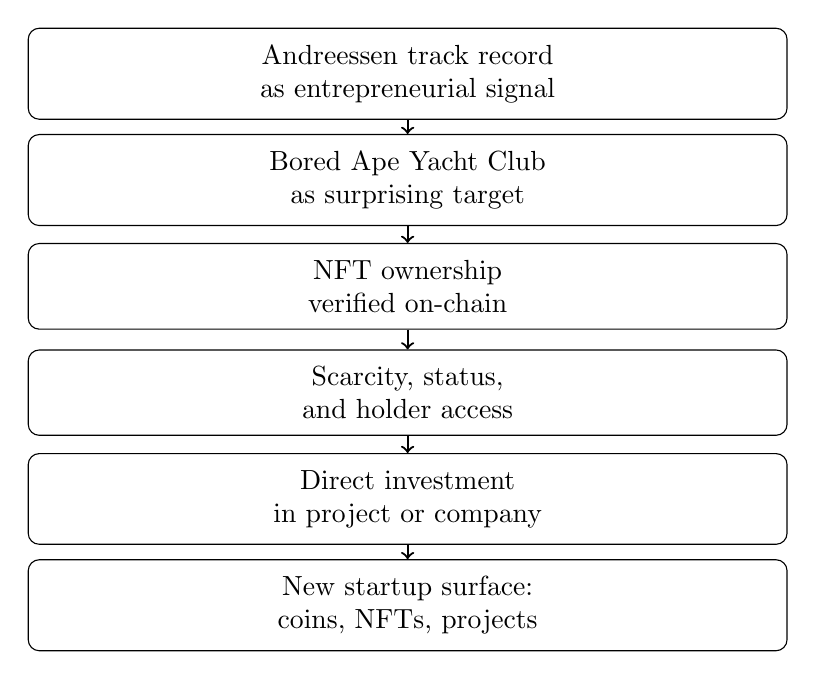
\begin{tikzpicture}[
  box/.style={
    draw,
    rounded corners,
    align=center,
    text width=0.76\linewidth,
    inner sep=6pt
  },
  arrow/.style={->, thick}
]
\node[box] (track) at (0,0) {Andreessen track record\\as entrepreneurial signal};
\node[box] (bayc) at (0,-1.35) {Bored Ape Yacht Club\\as surprising target};
\node[box] (verify) at (0,-2.70) {NFT ownership\\verified on-chain};
\node[box] (access) at (0,-4.05) {Scarcity, status,\\and holder access};
\node[box] (company) at (0,-5.40) {Direct investment\\in project or company};
\node[box] (startup) at (0,-6.75) {New startup surface:\\coins, NFTs, projects};

\draw[arrow] (track) -- (bayc);
\draw[arrow] (bayc) -- (verify);
\draw[arrow] (verify) -- (access);
\draw[arrow] (access) -- (company);
\draw[arrow] (company) -- (startup);
\end{tikzpicture}
\caption{A transcript-derived reconstruction of the lecture's sequence. There are no validated screenshot figures for this lecture, so the diagram is a conceptual reconstruction from the spoken argument.}
\end{figure}

\section{Asset Exposure Versus Company Exposure}

The second major pivot comes when the speaker brings the discussion back to Andreessen. Up to this point, the story is about buying an NFT and hoping that it appreciates or unlocks benefits. The new question is different: what if the serious capital goes not into the asset itself, but into the project or company behind the asset?

The lecture gives a claimed scale:
\begin{equation}
I_{\mathrm{Andreessen}} \sim \$4\mathrm{B} \text{ to } \$5\mathrm{B}.
\end{equation}
This should be read as a claim made in the lecture, not as a verified transaction figure. Its role is to mark the size of the move the speaker is trying to explain.

\subsection{Question \& Answer}

\paragraph{Question.}
What changes when the investment target is the NFT project or company rather than the NFT itself?

\paragraph{Answer.}
The exposure changes. Buying the NFT gives exposure to the asset: resale price, status, and holder benefits. Investing in the project or company gives exposure to the operating system around the assets: the brand, the community, the events, the software, the marketplace relationships, and whatever business model the founders build.

We can write the distinction as
\begin{align}
E_{\mathrm{asset}}
&\approx
\Delta P_{\mathrm{NFT}} + B_{\mathrm{holder}}, \\
E_{\mathrm{company}}
&\approx
R_{\mathrm{ecosystem}}.
\end{align}
Here \(E_{\mathrm{asset}}\) is asset exposure, \(\Delta P_{\mathrm{NFT}}\) is the change in resale value, and \(B_{\mathrm{holder}}\) represents holder benefits. By contrast, \(E_{\mathrm{company}}\) is project or company exposure, and \(R_{\mathrm{ecosystem}}\) denotes returns from the broader business built around the NFT ecosystem.

The point is not that one exposure is automatically better. The point is that they are different. The lecture's ``Pandora's box'' moment is the possibility that crypto investors may no longer be limited to buying coins or buying NFTs. They may also seek exposure to companies built around NFT communities.

\paragraph{Worked classification.}
Suppose we classify the investment choices mentioned in the lecture into a set
\begin{equation}
\mathcal{S}
=
\{\text{coin},\ \text{NFT asset},\ \text{NFT project/company}\}.
\end{equation}
A simple decision rule follows:

\begin{enumerate}
\item If the capital buys a cryptocurrency, classify the exposure as coin-market exposure.
\item If the capital buys a Bored Ape NFT, classify the exposure as asset appreciation plus holder benefits.
\item If the capital funds the project or company behind Bored Ape Yacht Club, classify the exposure as ecosystem or enterprise exposure.
\end{enumerate}

So the same broad category, crypto investing, contains three distinct objects:
\begin{equation}
\text{coin}
\neq
\text{NFT asset}
\neq
\text{NFT project/company}.
\end{equation}
That is the clean commercial distinction the chapter should preserve.

\begin{table}
\centering
\begin{tabular}{p{0.25\linewidth} p{0.30\linewidth} p{0.30\linewidth}}
\hline
\textbf{Target} & \textbf{What is owned} & \textbf{What value depends on} \\
\hline
Coin & A liquid crypto token & Market demand for the token \\
NFT asset & A verified digital asset & Resale value, status, and holder access \\
Project or company & Exposure to the venture behind the ecosystem & Execution, brand, community, and business model \\
\hline
\end{tabular}
\caption{A pocket-safe comparison of the three investment targets distinguished by the lecture.}
\end{table}

\section{Startup Surface Area}

The final part of the lecture widens the frame from one investment to a market design idea. If investors can buy coins, buy NFTs, and fund NFT-backed projects, then new platforms can appear to organize those choices. The speaker imagines a future interface where one can trade coins, trade NFTs, and choose among different NFT projects to fund.

We can represent the imagined allocation map as
\begin{equation}
A:
\text{investor capital}
\longrightarrow
(\text{coins},\ \text{NFT assets},\ \text{projects}).
\end{equation}
The menu expands from two obvious crypto choices to three:
\begin{align}
\mathcal{S}_{\mathrm{old}}
&=
\{\text{coins},\ \text{NFT assets}\}, \\
\mathcal{S}_{\mathrm{new}}
&=
\{\text{coins},\ \text{NFT assets},\ \text{NFT projects/companies}\}.
\end{align}

The transcript becomes unreliable in the last stretch, especially around examples involving hotel keys, private keys, playlists, and other utilities. We should therefore keep the stable claim and not overbuild the details. The stable claim is this: NFT ownership may be the entry point into a commercial system, and that system may itself become investable.

\begin{figure}
\centering
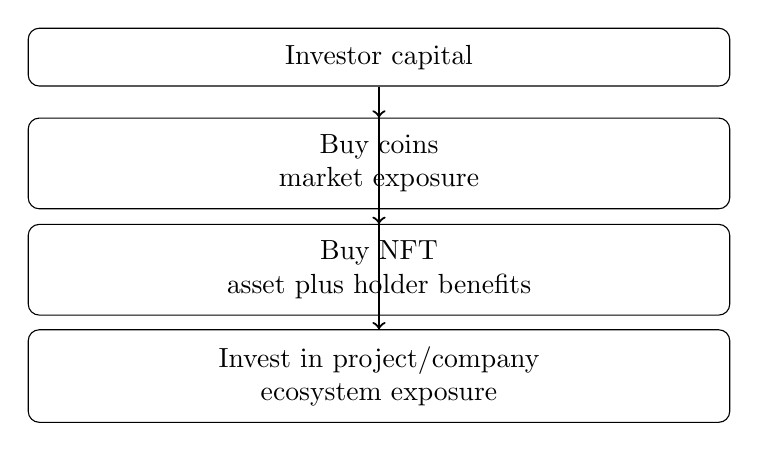
\begin{tikzpicture}[
  box/.style={
    draw,
    rounded corners,
    align=center,
    text width=0.70\linewidth,
    inner sep=6pt
  },
  arrow/.style={->, thick}
]
\node[box] (capital) at (0,0) {Investor capital};
\node[box] (coins) at (0,-1.35) {Buy coins\\market exposure};
\node[box] (nft) at (0,-2.70) {Buy NFT\\asset plus holder benefits};
\node[box] (project) at (0,-4.05) {Invest in project/company\\ecosystem exposure};

\draw[arrow] (capital) -- (coins);
\draw[arrow] (capital) -- (nft);
\draw[arrow] (capital) -- (project);
\end{tikzpicture}
\caption{The investment menu reconstructed from the lecture. The new category is project or company exposure, not merely token or NFT ownership.}
\end{figure}

\section{Summary}

The lecture unfolds in two questions. First, why should we care about this investor's move? Because the speaker treats Andreessen's track record as a signal. Second, why would that signal point toward a project built around monkey images? Because, in the lecture's business logic, the image is only the visible layer of a scarce, verifiable, socially recognized ownership system.

The final entrepreneurial distinction is between the asset and the structure behind the asset:
\begin{equation}
\text{verified ownership}
\longrightarrow
\text{exclusive access}
\longrightarrow
\text{project-level business}
\longrightarrow
\text{new startup surface}.
\end{equation}
That is the durable mechanism. The NFT is not just an object to trade. It can also be the entry credential for a community, a brand, and a company-level business system that outside capital may want to fund.